%-------------------------------------------------------------------------------------------------------
%-------------------------------------------------------------------------------------------------------
% Sec & Label

\section{Theoretical Analysis}
\label{sec:analysis}


%-------------------------------------------------------------------------------------------------------
%-------------------------------------------------------------------------------------------------------
% Intro

In this section, the Circuit T2 is analysed theoretically. In figure \ref{fig:Dsnh_oct_t2},
appart from all the components being identified, the assumed currents are also shown.
Only the node method was used in this section. Each subsection refers to each task.


Three important equations were used: both Kirchhoff's laws (Kirchhof's current law (KCL)
- eq.(\ref{eq:kcl}) and Kirchhoff's voltage law (KVL) - eq.(\ref{eq:kvl})); Ohm's law
(eq.(\ref{eq:ohm})).

The algebraic sum of all the currents in any given node is zero:
\begin{equation}
	\sum I_i = 0
	\label{eq:kcl}
\end{equation}

The algebraic sum of all the voltages in any given closed-loop circuit (mesh) is zero:
\begin{equation}
	\sum V_i = 0
	\label{eq:kvl}
\end{equation}

The potential difference between the two nodes connected to a resistor is equal to the current that 
passes through the resistor multiplied by its resistance.
\begin{equation}
	V_i = R_iI_i
	\label{eq:ohm}
\end{equation}

\begin{equation}
	V_1(t) = V_2(\infty) + [V_2(0) - V_2(\infty)]e^{\frac{-t}{\tau}}
\end{equation}



%-----------------------------------------------------------------------
%-----------------------------------------------------------------------
% 			      task1 - subsec
% ----------------------------------------------------------------------
% ----------------------------------------------------------------------
\subsection{Task 1)}
\label{subsec:task1_a}

When $t<0$ the value of $V_s$ is constant and so we can perform DC analysis on the circuit. We can assume that enough time has passed and so it is reasonable to assume that the circuit is in steady-state.

When performing a DC steady-state analysis on a circuit we can use the fact that the current flowing trough the capacitor is null (the circuit behaves as if the capacitor was removed).

A node analysis was performed to find the voltage value of each node and the current in each branch.

The node method uses KCL in conjunction with Ohm’s law to define equations that when solved give the voltage value 
of each nove in relation to ground (Node 4, $V_4 = 0$). 

In order to have equations that solve for the node’s voltage, a relation between curent and voltage is made using 
Ohm’s law (given a resistance between two nodes, the current that passes the resistance can be written as 
$I=\frac{V_2-V_1}{R_1}$)

To simplify the equations it is useful to use the conductance $G_n$ which is the inverse of the resistance $R_n$ 
($G_n=\frac{1}{R_n}$)

The equations used to solve the circuit were organized in matrix form.

{\footnotesize

$ \begin{bmatrix}
1 & 0 & 0 & 0 & 0 & 0 & 0 & 0 & 0 & 0 \\
G1 & -(G1+G2+G3) & G2 & G3 & 0 & 0 & 0 & 0 & 0 & 0 \\
0 & -G2 & G2 & 0 & 0 & 0 & 0 & 0 & -1 & 0 \\
0 & G3 & 0 & -(G3+G4+G5) & G5 & 0 & 0 & 0 & 0 & 0 \\
0 & 0 & 0 & -G5 & G5 & 0 & 0 & 0 & 1 & 1 \\
0 & 0 & 0 & 0 & 0 & G7 & -G7 & -1 & 0 & 1 \\
0 & 0 & 0 & 0 & 0 & -(G6+G7) & G7 & 0 & 0 & 0 \\
0 & 0 & 0 & 0 & 0 & 0 & 0 & 0 & 0 & 1 \\
0 & 0 & 0 & 1 & 0 & G6*K_d & -1 & 0 & 0 & 0 \\
0 & K_b & 0 & -K_b & 0 & 0 & 0 & 0 & -1 & 0 
\end{bmatrix}  $
$ \begin{bmatrix}
V1 \\
V2 \\
V3 \\
V5 \\
V6 \\
V7 \\
V8 \\
IH1 \\
Ib \\
Ic \\
\end{bmatrix}  $
=
$ \begin{bmatrix}
Vs\\
0\\
0\\
0\\
0\\
0\\
0\\
0\\
0\\
0\\
\end{bmatrix}  $
}

Figure \ref{fig:Desenho_t2}. In adition, assume $V_{Ni}$ to be the voltage in node $Ni$ (every node position can
also be found in Figure \ref{fig:Desenho_t2}). \\

\begin{figure}[ht]
	\centering
	\includegraphics[width=0.75\linewidth]{dsnh_oct_t2_al1.pdf}
	\caption{Circuit T2, analysed by Ngspice}
\label{fig:Dsnh_sim_t2}
\end{figure}






{\footnotesize

$ \begin{bmatrix}
1 & 0 & 0 & 0 & 0 & 0 & 0 & 0 & 0 & 0 \\
G1 & -(G1+G2+G3) & G2 & G3 & 0 & 0 & 0 & 0 & 0 & 0 \\
0 & -G2 & G2 & 0 & 0 & 0 & 0 & 0 & -1 & 0 \\
0 & G3 & 0 & -(G3+G4+G5) & G5 & 0 & 0 & 0 & 0 & 0 \\
0 & 0 & 0 & -G5 & G5 & 0 & 0 & 0 & 1 & 1 \\
0 & 0 & 0 & 0 & 0 & G7 & -G7 & -1 & 0 & 1 \\
0 & 0 & 0 & 0 & 0 & -(G6+G7) & G7 & 0 & 0 & 0 \\
0 & 0 & 0 & 0 & 0 & 0 & 0 & 0 & 0 & 1 \\
0 & 0 & 0 & 1 & 0 & G6*K_d & -1 & 0 & 0 & 0 \\
0 & K_b & 0 & -K_b & 0 & 0 & 0 & 0 & -1 & 0 
\end{bmatrix}  $
$ \begin{bmatrix}
V1 \\
V2 \\
V3 \\
V5 \\
V6 \\
V7 \\
V8 \\
IH1 \\
Ib \\
Ic \\
\end{bmatrix}  $
=
$ \begin{bmatrix}
V1 \\
V2 \\
V3 \\
V5 \\
V6 \\
V7 \\
V8 \\
IH1 \\
Ib \\
Ic \\
\end{bmatrix}  $
}

{\footnotesize

$ \begin{bmatrix}
1 & 0 & 0 & 0 & 0 & 0 & 0 & 0 & 0 & 0 \\
G1 & -(G1+G2+G3) & G2 & G3 & 0 & 0 & 0 & 0 & 0 & 0 \\
0 & -G2 & G2 & 0 & 0 & 0 & 0 & 0 & -1 & 0 \\
0 & G3 & 0 & -(G3+G4+G5) & G5 & 0 & 0 & 0 & 0 & 0 \\
0 & 0 & 0 & -G5 & G5 & 0 & 0 & 0 & 1 & 1 \\
0 & 0 & 0 & 0 & 0 & G7 & -G7 & -1 & 0 & 1 \\
0 & 0 & 0 & 0 & 0 & -(G6+G7) & G7 & 0 & 0 & 0 \\
0 & 0 & 0 & 0 & 1 & 0 & -1 & 0 & 0 & 0 \\
0 & 0 & 0 & 1 & 0 & G6*K_d & -1 & 0 & 0 & 0 \\
0 & Kb & 0 & -K_b & 0 & 0 & 0 & 0 & -1 & 0 
\end{bmatrix}  $
$ \begin{bmatrix}
V1 \\
V2 \\
V3 \\
V5 \\
V6 \\
V7 \\
V8 \\
IH1_2 \\
Ib_2 \\
Ic_2 \\
\end{bmatrix}  $
=
$ \begin{bmatrix}
V1 \\
V2 \\
V3 \\
V5 \\
V6 \\
V7 \\
V8 \\
IH1 \\
Ib \\
Ic \\
\end{bmatrix}  $

$ \begin{bmatrix}
1 & 0 & 0 & 0 & 0 & 0 & 0 & 0 & 0 & 0 \\
G1 & -(G1+G2+G3) & G2 & G3 & 0 & 0 & 0 & 0 & 0 & 0 \\
0 & -G2 & G2 & 0 & 0 & 0 & 0 & 0 & -1 & 0 \\
0 & G3 & 0 & -(G3+G4+G5) & G5 & 0 & 0 & 0 & 0 & 0 \\
0 & 0 & 0 & -G5 & G5 & 0 & 0 & 0 & 1 & 1 \\
0 & 0 & 0 & 0 & 0 & G7 & -G7 & -1 & 0 & 1 \\
0 & 0 & 0 & 0 & 0 & -(G6+G7) & G7 & 0 & 0 & 0 \\
0 & 0 & 0 & 0 & -1/Z_c & 0 & 1/Z_c & 0 & 0 & 0 \\
0 & 0 & 0 & 1 & 0 & G6*K_d & -1 & 0 & 0 & 0 \\
0 & K_b & 0 & -K_b & 0 & 0 & 0 & 0 & -1 & 0 
\end{bmatrix}  $
$ \begin{bmatrix}
V1_3 \\
V2_3 \\
V3_3 \\
V5_3 \\
V6_3 \\
V7_3 \\
V8_3 \\
\end{bmatrix}  $
=
$ \begin{bmatrix}
V1 \\
V2 \\
V3 \\
V5 \\
V6 \\
V7 \\
V8 \\
IH1 \\
Ib \\
Ic \\
\end{bmatrix}  $
}

With these 8 equations it is possible to solve the system using Octave.
The results were organized in Table \ref{tab:node}

\begin{table}[ht]
	\centering
	\begin{tabular}{|l|r|}
    		\hline    
    		{\bf Name} & {\bf Value [A or V]} \\ \hline
    		$V_{N1}$ & 5.114025e+00 \\ \hline 
$V_{N2}$ & 4.830792e+00 \\ \hline 
$V_{N3}$ & 4.226624e+00 \\ \hline 
$V_{N5}$ & 4.871651e+00 \\ \hline 
$V_{N6}$ & 5.781844e+00 \\ \hline 
$V_{N7}$ & -1.849204e+00 \\ \hline 
$V_{N8}$ & -2.786253e+00 \\ \hline 
$@I_{b}$ & -2.957272e-04 \\ \hline 
$@I_{c}$ & 0.000000e+00 \\ \hline 
$@I_{R1}$ & 2.822201e-04 \\ \hline 
$@I_{R2}$ & -2.957272e-04 \\ \hline 
$@I_{R3}$ & -1.350709e-05 \\ \hline 
$@I_{R4}$ & 1.200956e-03 \\ \hline 
$@I_{R5}$ & -2.957272e-04 \\ \hline 
$@I_{d}$ & -9.187358e-04 \\ \hline 
$@I_{R6}$ & 9.187358e-04 \\ \hline 

  	\end{tabular}
  	\caption{Values computed by Octave. Variables identified with a '$@$' have a
  	corresponding value in Ampere (A). The others are expressed in Volts (V).}
 
\label{tab:node}
\end{table}

%-----------------------------------------------------------------------
%-----------------------------------------------------------------------
% 			      task2 - subsec
% ----------------------------------------------------------------------
% ----------------------------------------------------------------------
\subsection{Task 2)}
\label{subsec:task2_a}

In this section the capacitor is replaced with a voltage source $V_x$ with value $V_x = V_6 - V_8$ as shown in figure.... The same type of analysis was made to this circuit but with a slightly modification on some of the rows to represent the modified circuit.

Tabela-------------


By performing this analysis we can compute the current $I_x$ that flows trough $V_s$. Using Ohm's law we can calculate the equivente resistance $R_{eq}$:

\[
R_{eq}=\frac{V_x}{I_x}
\]


This procedure is important to compute the circuit's time constant $\tau$ by using the equation $\tau = CR_{eq}$. The time constant in conjunction with the boundary conditions of the circuit are required to compute the natural solution of the circuit.


\begin{figure}[ht]
	\centering
	\includegraphics[width=0.75\linewidth]{dsnh_oct_t2_al2.pdf}
	\caption{Circuit T2, analysed by Ngspice}
\label{fig:Dsnh_sim_t2}
\end{figure}

%-----------------------------------------------------------------------
%-----------------------------------------------------------------------
% 			      task3 - subsec
% ----------------------------------------------------------------------
% ----------------------------------------------------------------------
\subsection{Task 3)}
\label{subsec:task3_a}

With the circuit's time constant $\tau$ and boundary conditions calculated in the previous task we can use following equation to get the natural solution of the circuit:

\[
V_{6n}(t) = V_6(\infty) + [V_6(0) - V_6(\infty)]e^{\frac{-t}{\tau}}
\] 

Since $V_s$ is considered to be null on this circuit, the value of node 6 is 0 at infinity $V_6(\infty) = 0$ 


\begin{figure}[ht]
	\centering
	\includegraphics[width=0.75\linewidth]{dsnh_oct_t2_al3.pdf}
	\caption{Circuit T2, analysed by Ngspice}
\label{fig:Dsnh_sim_t2}
\end{figure}

\begin{figure}[ht]
	\centering
	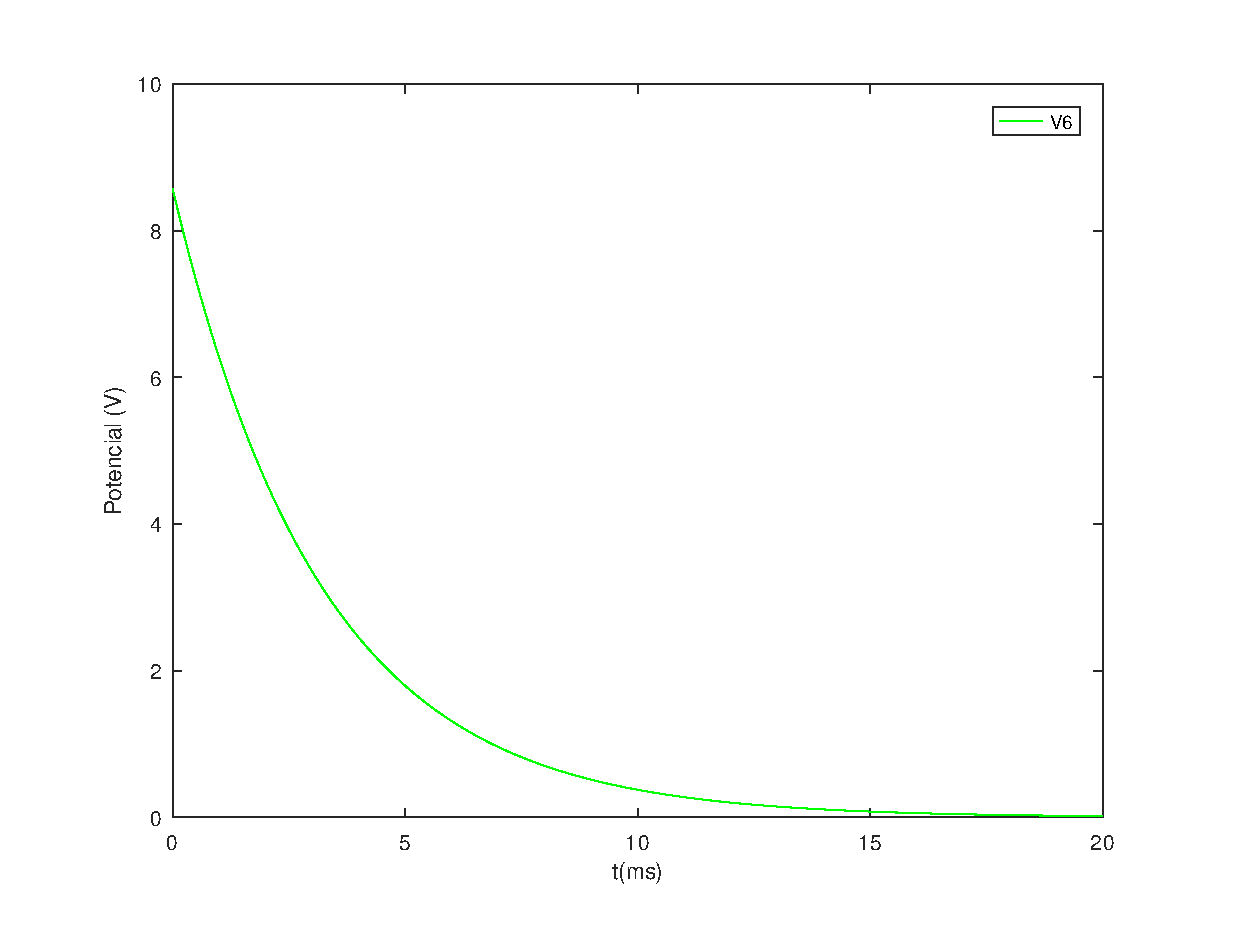
\includegraphics[width=0.55\linewidth]{plot1.eps}
	\caption{Plot oct - 1}
\label{fig:Dsnh_sim_t2}
\end{figure}

%-----------------------------------------------------------------------
%-----------------------------------------------------------------------
% 			      task4 - subsec
% ----------------------------------------------------------------------
% ----------------------------------------------------------------------
\subsection{Task 4)}
\label{subsec:task4_a}

In this task the forced solution of the circuit is computed. To acomplish this objetive, we do an analysis using a phasor voltage source $V_s=1$ and replacing C with its impedance:

\[
Z_c = j\frac{1}{C\omega}
\]

Doing an analysis similar to the previous ones, with a slightly modified matrix we can determine the phasor voltages in all nodes.

The following table shows the phasor magnitudes in each node.


\begin{figure}[ht]
	\centering
	\includegraphics[width=0.75\linewidth]{dsnh_oct_t2_al456.pdf}
	\caption{Circuit T2, analysed by Ngspice}
\label{fig:Dsnh_sim_t2}
\end{figure}

%-----------------------------------------------------------------------
%-----------------------------------------------------------------------
% 			      task5 - subsec
% ----------------------------------------------------------------------
% ----------------------------------------------------------------------
\subsection{Task 5)}
\label{subsec:task5_a}

In this task we compute the final total solution $v_6(t)$ with a frequncy of 1000Hz. To achieve the final result the phasors are converted to real time functions and than superimposed with the natural solution found before.

The force solution will have the form:

\[
V_{6f}(t) = V*sin(\omega t + \phi)
\]

The constant $\omega$ is the angular frequency of the voltage source, $V$ is the amplitude of the node phasor and $\phi$ is the phase shift of the node phasor.

The final solution will have the form:

\[
V_6(t) = V_{6n} + V_{6f}
\]

The following graph plots the results computed by octave in interval [-5, 20]ms.

\begin{figure}[ht]
	\centering
	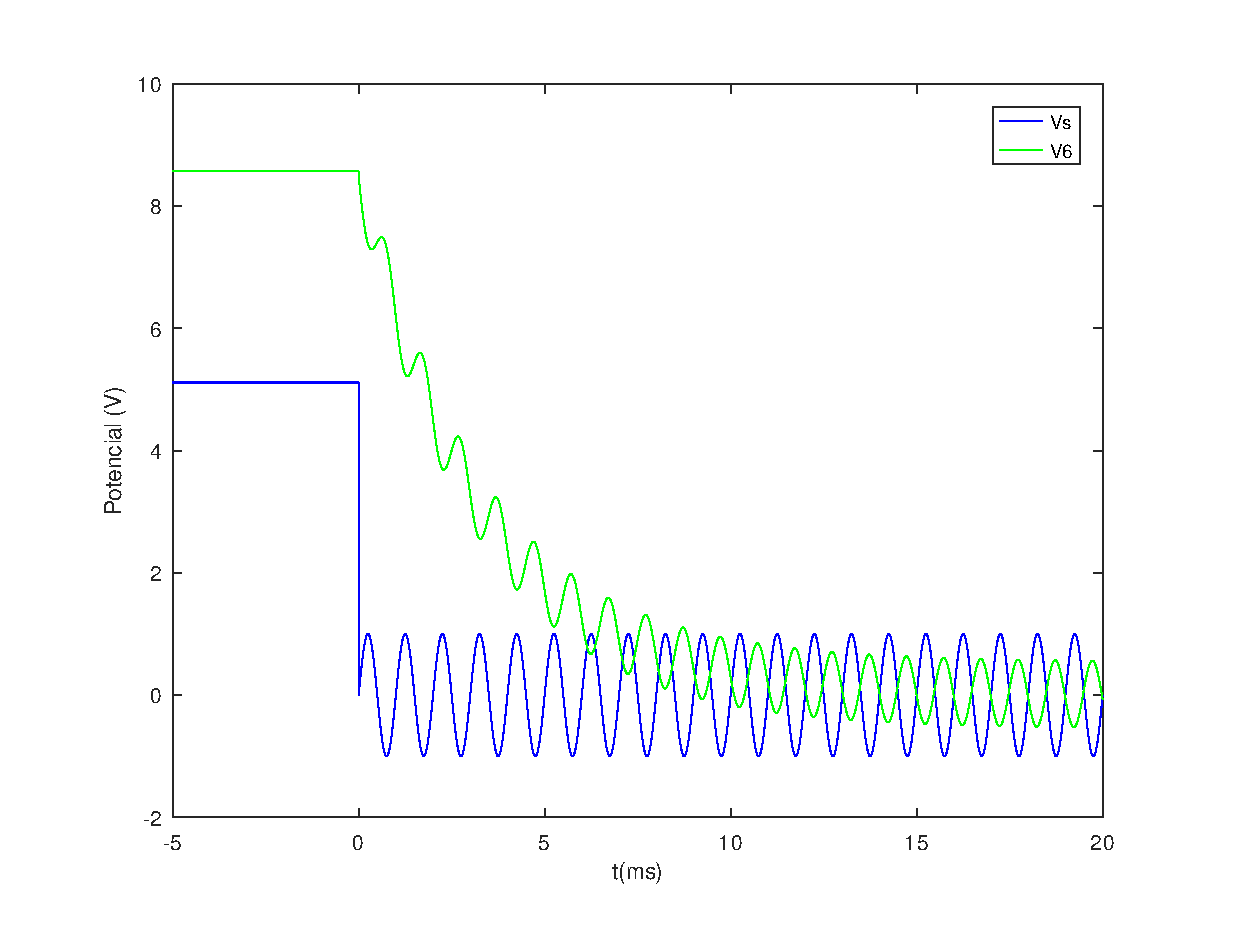
\includegraphics[width=0.55\linewidth]{plot2.eps}
	\caption{Plot oct - 2}
\label{fig:Dsnh_sim_t2}
\end{figure}

%-----------------------------------------------------------------------
%-----------------------------------------------------------------------
% 			      task6 - subsec
% ----------------------------------------------------------------------
% ----------------------------------------------------------------------
\subsection{Task 6)}
\label{subsec:task6_a}

In this task, the frequency response of $v_c(f)= v_6(f) - v_8(f)$ and $v_6(f)$ is determined for a frequency range of 0.1Hz to 1 MHz. For the calculation of the frequecy response a similar analysis to the one in task 4) was made for a multitude of frequencys in the set the frequency range. The following graph shows the achieved results: 


Grafico-----------


We can see that the value of $v_c(f)$ in dB decreases with increasing frequency. This behaviour is due to the impedance of the capacitor decreasing with larger frequencies and so the phasor voltage difference tends to zero (since the magnitude is ploted in dB, when a voltage approaches 0 the dB values goes to negative values).

The value of $v_c(f)$ also decreases for the same reasons explained in subsection 2.5).




\begin{figure}[ht]
	\centering
	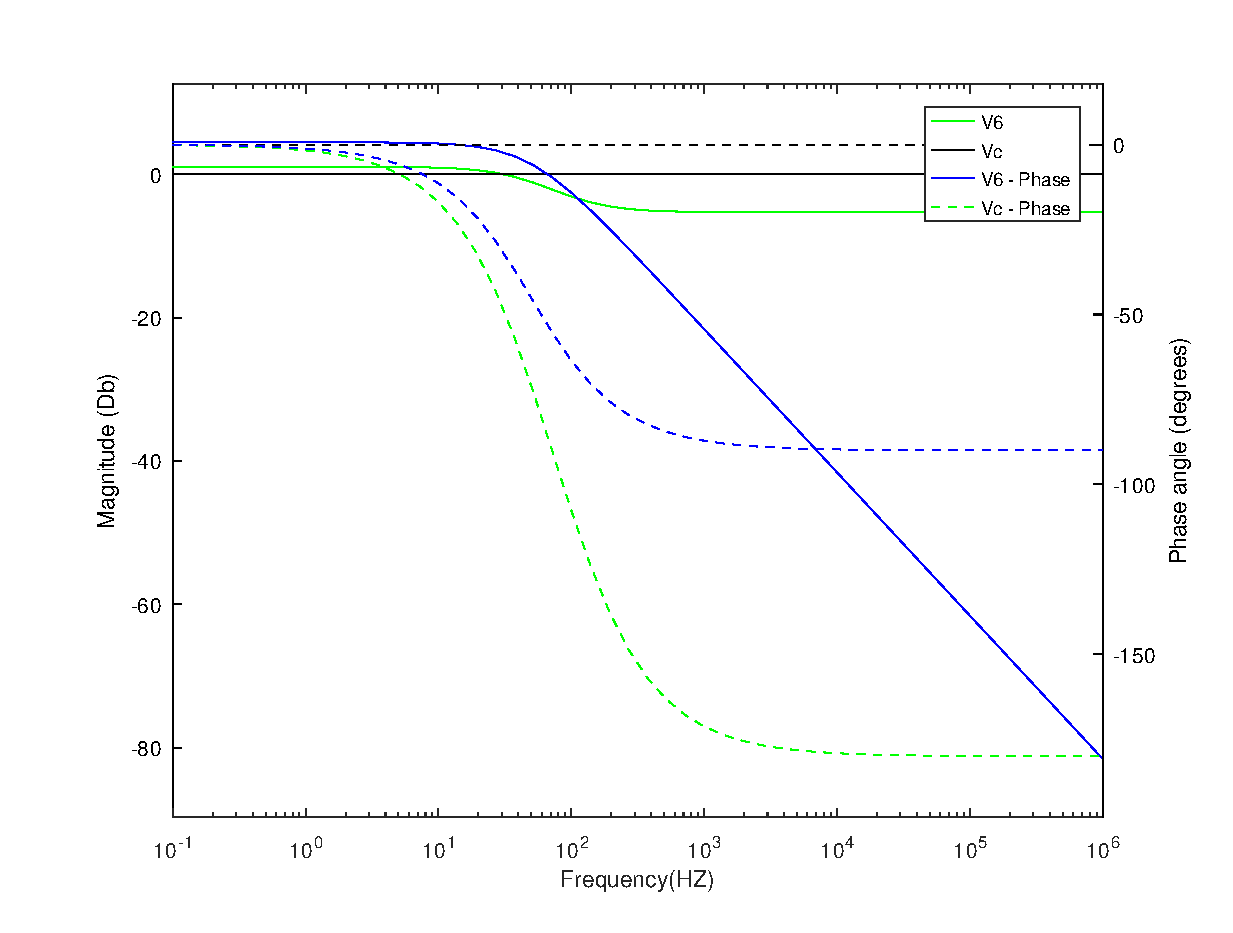
\includegraphics[width=0.55\linewidth]{plot3.eps}
	\caption{Plot oct - 3}
\label{fig:Dsnh_sim_t2}
\end{figure}



